\documentclass[a4j,12pt]{jarticle}
\usepackage[dvips]{graphicx}
\usepackage{okumacro, cite, url}
\usepackage{ascmac, comment, color, multirow, ifthen, mediabb}
\usepackage{cover, graduation}

\newcounter{ChangedColor}
% 1: 変更箇所に赤色を付ける
% 0: 変更箇所に赤色を付けない
\setcounter{ChangedColor}{1}

\ifthenelse{\equal{\theChangedColor}{0}} %
           {\newcommand{\Ca}[1]{#1}} %
           {\newcommand{\Ca}[1]{\textcolor{red}{#1}}} %

\年度{2019}
\学期{秋}
\クラス{○○}
\卒研題目{○○○○○○○○○○○○○○ \\ ○○○○○○○○○○○○}
\氏名{○○ ○○}
\回生{4}
\学籍番号{2600000000-0}
\指導教員{毛利 公一 教授}
\提出日{2023年1月31日}

\begin{document}
\makecoverpage
\clearpage

\setlength{\baselineskip}{20pt}	% 行間の設定
\pagestyle{empty}

\section*{内容梗概}
本論文をまとめましょう
			% 内容梗概

\pagenumbering{roman}
\pagestyle{plain}
% 目次(行間を修正して1ページに納めたいなどはこちら)
{\setlength{\baselineskip}{17.2pt} \tableofcontents}
%\tableofcontents			% 目次
\clearpage
\listoffigures				% 図目次
\listoftables				% 表目次
\clearpage
\pagenumbering{arabic}

% 以下,各章のファイルをincludeする
\section{はじめに}
はじめには,2ページを目安に書きましょう.
参考文献はbibtexを使いましょう.普段からゼミで使用している人は,referencesファイルを自分のものに
置き換えてください.
bibtexの使い方は,references.bibを作り,\verb|\cite{jmoni}|の様に本文で参照\cite{jmoni}し,
jbibtexコマンドでさくっとできます.
論文データベースには,必ずbibtex形式というのが用意されているはず.
その内容をコピーすれば基本は大丈夫.
参考文献のスタイルは,情報処理学会の出現順のものを使用しています.
			% はじめに
\section{図の挿入方法}
EPSは図\ref{fig:eps}のように入れられます.
章タイトルの上に図が来ることがないように.

\begin{figure}[hb]
    \centering
    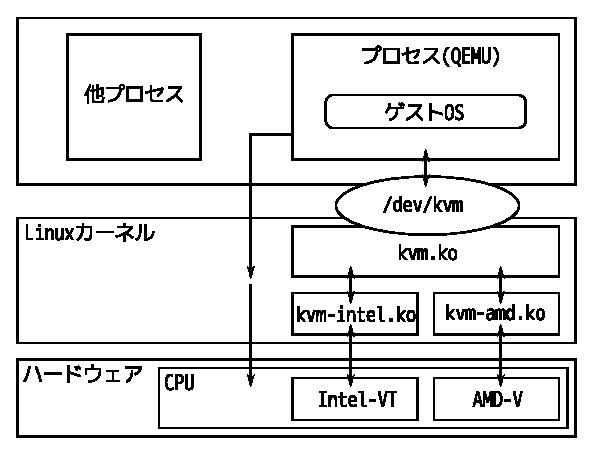
\includegraphics[width=\columnwidth,keepaspectratio]{fig/kvm-and-qemu-arch.eps}
    \caption{キャプション}
    \label{fig:eps}
\end{figure}
  		% 図挿入の例


\section*{謝辞}
  		% 謝辞
% 参考文献はbibtexを使いましょう
\AddTableOfContents{参考文献}
\bibliography{references}
\bibliographystyle{ipsjunsrt}
\end{document}
